\documentclass[11pt,a4paper]{report}
\usepackage[textwidth=37em,vmargin=30mm]{geometry}
\usepackage{calc,xunicode,amsmath,amssymb,paralist,enumitem,tabu,booktabs,datetime2,xeCJK,xeCJKfntef,listings}
\usepackage{tocloft,fancyhdr,tcolorbox,xcolor,graphicx,eso-pic,xltxtra,xelatexemoji}

\newcommand{\envyear}[0]{2025}
\newcommand{\envdatestr}[0]{2025-01-14}
\newcommand{\envfinaldir}[0]{webdb/2025/20250114/final}

\usepackage[hidelinks]{hyperref}
\hypersetup{
    colorlinks=false,
    pdfpagemode=FullScreen,
    pdftitle={Web Digest - \envdatestr}
}

\setlength{\cftbeforechapskip}{10pt}
\renewcommand{\cftchapfont}{\rmfamily\bfseries\large\raggedright}
\setlength{\cftbeforesecskip}{2pt}
\renewcommand{\cftsecfont}{\sffamily\small\raggedright}

\setdefaultleftmargin{2em}{2em}{1em}{1em}{1em}{1em}

\usepackage{xeCJK,xeCJKfntef}
\xeCJKsetup{PunctStyle=plain,RubberPunctSkip=false,CJKglue=\strut\hskip 0pt plus 0.1em minus 0.05em,CJKecglue=\strut\hskip 0.22em plus 0.2em}
\XeTeXlinebreaklocale "zh"
\XeTeXlinebreakskip = 0pt


\setmainfont{Brygada 1918}
\setromanfont{Brygada 1918}
\setsansfont{IBM Plex Sans}
\setmonofont{JetBrains Mono NL}
\setCJKmainfont{Noto Serif CJK SC}
\setCJKromanfont{Noto Serif CJK SC}
\setCJKsansfont{Noto Sans CJK SC}
\setCJKmonofont{Noto Sans CJK SC}

\setlength{\parindent}{0pt}
\setlength{\parskip}{8pt}
\linespread{1.15}

\lstset{
	basicstyle=\ttfamily\footnotesize,
	numbersep=5pt,
	backgroundcolor=\color{black!5},
	showspaces=false,
	showstringspaces=false,
	showtabs=false,
	tabsize=2,
	captionpos=b,
	breaklines=true,
	breakatwhitespace=true,
	breakautoindent=true,
	linewidth=\textwidth
}






\newcommand{\coverpic}[2]{
    % argv: itemurl, authorname
    Cover photo by #2~~(\href{#1}{#1})
}
\newcommand{\makeheader}[0]{
    \begin{titlepage}
        % \newgeometry{hmargin=15mm,tmargin=21mm,bmargin=12mm}
        \begin{center}
            
            \rmfamily\scshape
            \fontspec{BaskervilleF}
            \fontspec{Old Standard}
            \fontsize{59pt}{70pt}\selectfont
            WEB\hfill DIGEST
            
            \vfill
            % \vskip 30pt
            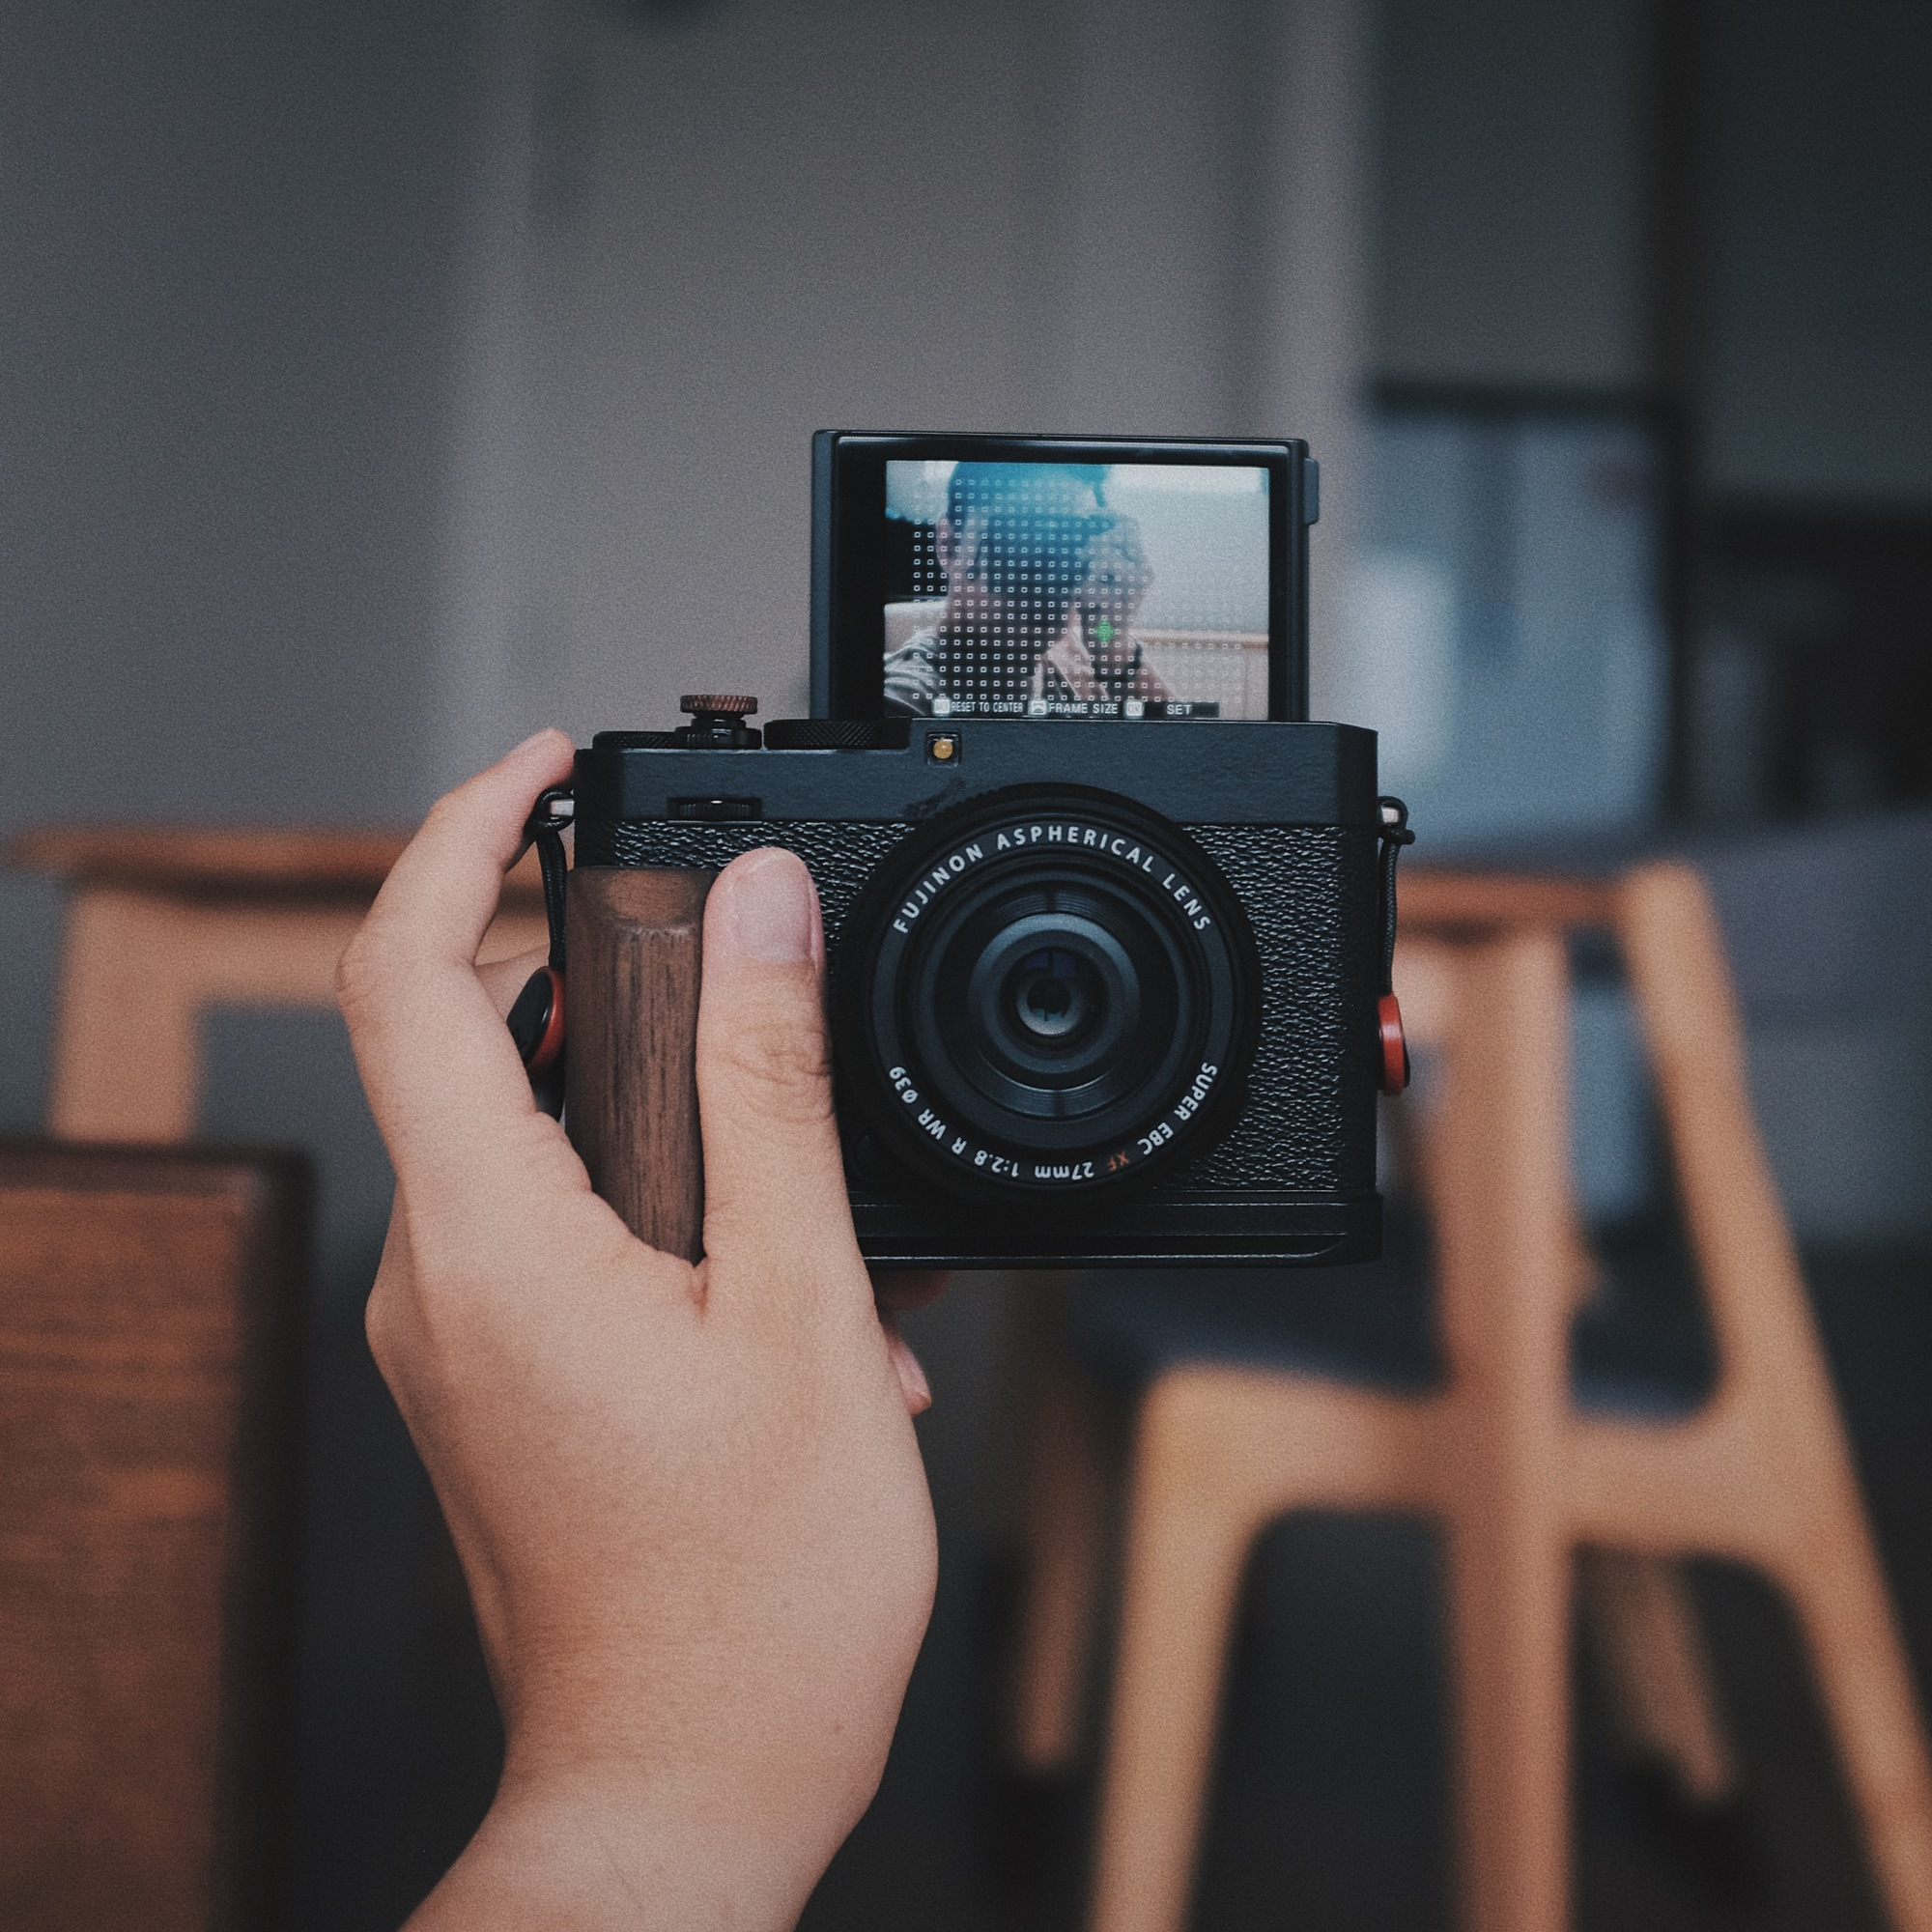
\includegraphics[width=\linewidth]{\envfinaldir/coverpic-prod.jpg}\par
            % \vskip 30pt
            \vfill

            \normalsize\rmfamily\scshape
            \copyright{} The Web Digest Project \hfill\large \envdatestr
        \end{center}
    \end{titlepage}
    % \restoregeometry
}
\newcommand{\simplehref}[1]{%
    \textcolor{blue!80!green}{\href{#1}{#1}}%
}
\renewcommand{\contentsname}{\center\Huge\sffamily\bfseries Contents\par\vskip 20pt}
\newcounter{ipartcounter}
\setcounter{ipartcounter}{0}
\newcommand{\ipart}[1]{
    % \vskip 20pt
    \clearpage
    \stepcounter{ipartcounter}
    \phantomsection
    \addcontentsline{toc}{chapter}{#1}
    % \begin{center}
    %     \Huge
    %     \sffamily\bfseries
    %     #1
    % \end{center}
    % \vskip 20pt plus 7pt
}
\newcounter{ichaptercounter}
\setcounter{ichaptercounter}{0}
\newcommand{\ichapter}[1]{
    % \vskip 20pt
    \clearpage
    \stepcounter{ichaptercounter}
    \phantomsection
    \addcontentsline{toc}{section}{\numberline{\arabic{ichaptercounter}}#1}
    \begin{center}
        \Huge
        \sffamily\bfseries
        #1
    \end{center}
    \vskip 20pt plus 7pt
}
\newcommand{\entrytitlefont}[1]{\subsection*{\raggedright\Large\sffamily\bfseries#1}}
\newcommand{\entryitemGeneric}[2]{
    % argv: title, url
    \parbox{\linewidth}{
        \entrytitlefont{#1}\par\vskip 5pt
        \footnotesize\ttfamily\mdseries
        \simplehref{#2}
    }\vskip 11pt plus 11pt minus 1pt
}
\newcommand{\entryitemGithub}[3]{
    % argv: title, url, desc
    \parbox{\linewidth}{
        \entrytitlefont{#1}\par\vskip 5pt
        \footnotesize\ttfamily\mdseries
        \simplehref{#2}\par\vskip 5pt
        \small\rmfamily\mdseries#3
    }\vskip 11pt plus 11pt minus 1pt
}
\newcommand{\entryitemAp}[3]{
    % argv: title, url, desc
    \parbox{\linewidth}{
        \entrytitlefont{#1}\par\vskip 5pt
        \footnotesize\ttfamily\mdseries
        \simplehref{#2}\par\vskip 5pt
        \small\rmfamily\mdseries#3
    }\vskip 11pt plus 11pt minus 1pt
}
\newcommand{\entryitemHackernews}[3]{
    % argv: title, hnurl, rawurl
    % \parbox{\linewidth}{
    %     \entrytitlefont{#1}\par\vskip 5pt
    %     \footnotesize\ttfamily\mdseries
    %     \simplehref{#3}\par
    %     \textcolor{black!50}{\href{#2}{#2}}
    % }\vskip 11pt plus 11pt minus 1pt
    \begin{minipage}{\linewidth}
            \entrytitlefont{#1}\par\vskip 5pt
            \footnotesize\ttfamily\mdseries
            \simplehref{#3}\par
            \textcolor{black!50}{\href{#2}{#2}}
    \end{minipage}\par\vskip 11pt plus 11pt minus 1pt
}







\begin{document}

\makeheader

\tableofcontents\clearpage




\ipart{Developers}
\ichapter{Hacker News}
\entryitemTwoLinks{JPMorgan Workers Ponder Union in Wake of Return-to-Office Mandate}{https://news.ycombinator.com/item?id=42688159}{https://www.barrons.com/articles/jpmorgan-back-to-office-mandate-union-4206af78}

\entryitemTwoLinks{Sonos CEO steps down after app update debacle}{https://news.ycombinator.com/item?id=42687932}{https://www.reuters.com/business/retail-consumer/sonos-ceo-patrick-spence-steps-down-after-app-update-debacle-2025-01-13/}

\entryitemTwoLinks{WordPress Is in Trouble}{https://news.ycombinator.com/item?id=42687121}{https://anderegg.ca/2025/01/11/wordpress-is-in-trouble}

\entryitemTwoLinks{AI Engineer Reading List}{https://news.ycombinator.com/item?id=42686457}{https://www.latent.space/p/2025-papers}

\entryitemTwoLinks{Let's Quit X}{https://news.ycombinator.com/item?id=42686362}{https://www.helloquitx.com}

\entryitemTwoLinks{Why Skyscrapers Became Glass Boxes}{https://news.ycombinator.com/item?id=42683736}{https://www.construction-physics.com/p/why-skyscrapers-became-glass-boxes}

\entryitemTwoLinks{Luck Be a Landlord Might Be Banned from Google Play}{https://news.ycombinator.com/item?id=42683567}{https://blog.trampolinetales.com/luck-be-a-landlord-might-be-banned-from-google-play-2/}

\entryitemTwoLinks{Fluid Simulation Pendant}{https://news.ycombinator.com/item?id=42683389}{https://mitxela.com/projects/fluid-pendant}

\entryitemTwoLinks{Literate programming: Knuth is doing it wrong (2014)}{https://news.ycombinator.com/item?id=42683009}{https://akkartik.name/post/literate-programming}

\entryitemTwoLinks{Live London Underground / bus maps taken down by TfL trademark complaint}{https://news.ycombinator.com/item?id=42682876}{https://traintimes.org.uk/map/tube/}

\entryitemTwoLinks{Ask HN: Am I the only one here who can't stand HN's AI obsession?}{https://news.ycombinator.com/item?id=42682821}{https://news.ycombinator.com/item?id=42682821}

\entryitemTwoLinks{Can you complete the Oregon Trail if you wait at river for 14272 years: A study}{https://news.ycombinator.com/item?id=42682813}{https://moral.net.au/writing/2025/01/11/waiting\_for\_oregon/}

\entryitemTwoLinks{Euro-cloud provider Anexia moves 12,000 VMs off VMware to homebrew KVM platform}{https://news.ycombinator.com/item?id=42682671}{https://www.theregister.com/2025/01/13/anexia\_vmware\_to\_kvm\_migration/}

\entryitemTwoLinks{Debugging: Indispensable rules for finding even the most elusive problems (2004)}{https://news.ycombinator.com/item?id=42682602}{https://dwheeler.com/essays/debugging-agans.html}

\entryitemTwoLinks{The Origins of Wokeness}{https://news.ycombinator.com/item?id=42682305}{https://paulgraham.com/woke.html}

\entryitemTwoLinks{Vanished from Google/Bing/LinkedIn: a rebuttal of an anti-net neutrality paper}{https://news.ycombinator.com/item?id=42681240}{http://internetthought.blogspot.com/2025/01/vanished-from-index-of-google-bing-and.html}

\entryitemTwoLinks{Facebook blocks links to Pixelfed, a federated Instagram alternative}{https://news.ycombinator.com/item?id=42680769}{https://bsky.app/profile/did:plc:n2okvbdq33c32ekbv6hfzdg2/post/3lfjk3mrdds23}

\entryitemTwoLinks{Blue Origin New Glenn Mission NG-1 – Live}{https://news.ycombinator.com/item?id=42680510}{https://www.blueorigin.com}

\entryitemTwoLinks{Show HN: New search engine and free-FOIA-by-fax-via-web for US veteran records}{https://news.ycombinator.com/item?id=42680048}{https://www.birls.org}

\entryitemTwoLinks{Disco Elysium Explorer}{https://news.ycombinator.com/item?id=42679679}{http://134.0.119.41}\ichapter{Phoronix}
\entryitemGeneric{\hskip 0pt{}Intel Battlemage Showing Off Nice OpenCL Gains With Newest Open-Source Compute Stack}{https://www.phoronix.com/review/intel-b580-opencl-january}

\entryitemGeneric{\hskip 0pt{}Oracle OLED Wants To Help Improve The Debugability Of The Linux Kernel}{https://www.phoronix.com/news/Oracle-Linux-OLED-Debug}

\entryitemGeneric{\hskip 0pt{}GNOME Shell 48 Alpha Introduces Screen Time / Health Breaks, Mutter 48 Alpha Out Too}{https://www.phoronix.com/news/GNOME-Shell-Muter-48-Alpha}

\entryitemGeneric{\hskip 0pt{}DXVK 2.5.3 Brings More Fixes For Direct3D 9 / 10 / 11 On Vulkan}{https://www.phoronix.com/news/DXVK-2.5.3-Released}

\entryitemGeneric{\hskip 0pt{}Linux Attack Vector Controls Updated To More Easily Controlling CPU Security Mitigations}{https://www.phoronix.com/news/Linux-CPU-Attack-Vector-Control}

\entryitemGeneric{\hskip 0pt{}A Microsoft-Contributed Change To Linux 6.13 Is Causing A Last Minute Ruckus}{https://www.phoronix.com/news/Linux-6.13-Dropping-EXECMEM\_ROX}

\entryitemGeneric{\hskip 0pt{}Alibaba Engineers Work To Address Suspend/Resume Bugs With The AMD Graphics Driver}{https://www.phoronix.com/news/Alibaba-AMDGPU-Suspend-Resume}

\entryitemGeneric{\hskip 0pt{}Intel Gigabit Ethernet Driver To Speed-Up With AF\_XDP Zero-Copy For Linux 6.14}{https://www.phoronix.com/news/IntelIGB-AF-XDP-Zero-Copy}

\entryitemGeneric{\hskip 0pt{}AMD Broadcast TLB Invalidation Linux Patches Reworked In 4th Spin}{https://www.phoronix.com/news/AMD-INVLPGB-Linux-v4-Patches}\ichapter{Dribbble}
\entryitemGeneric{\hskip 0pt{}Faith Education Icons}{https://dribbble.com/shots/25422138-Faith-Education-Icons}

\entryitemGeneric{\hskip 0pt{}Round Robin}{https://dribbble.com/shots/25467606-Round-Robin}

\entryitemGeneric{\hskip 0pt{}Learning App Design}{https://dribbble.com/shots/25458950-Learning-App-Design}

\entryitemGeneric{\hskip 0pt{}Cub Studio Process}{https://dribbble.com/shots/25456521-Cub-Studio-Process}

\entryitemGeneric{\hskip 0pt{}Polar Bear + Baby (2012)}{https://dribbble.com/shots/25454483-Polar-Bear-Baby-2012}

\entryitemGeneric{\hskip 0pt{}SHOWREEL 24'}{https://dribbble.com/shots/25450148-SHOWREEL-24}

\entryitemGeneric{\hskip 0pt{}Southland Provisions}{https://dribbble.com/shots/25456279-Southland-Provisions}

\entryitemGeneric{\hskip 0pt{}Cromatic.bio®}{https://dribbble.com/shots/25451539-Cromatic-bio}

\entryitemGeneric{\hskip 0pt{}Running Dog Logo}{https://dribbble.com/shots/25450403-Running-Dog-Logo}

\entryitemGeneric{\hskip 0pt{}Business set}{https://dribbble.com/shots/25444987-Business-set}

\entryitemGeneric{\hskip 0pt{}Pageless Logo \& Visual Identity}{https://dribbble.com/shots/25450527-Pageless-Logo-Visual-Identity}

\entryitemGeneric{\hskip 0pt{}REV Graphic Style}{https://dribbble.com/shots/25452261-REV-Graphic-Style}

\entryitemGeneric{\hskip 0pt{}B}{https://dribbble.com/shots/25449124-B}

\entryitemGeneric{\hskip 0pt{}Hive}{https://dribbble.com/shots/25452363-Hive}

\entryitemGeneric{\hskip 0pt{}Tempest Logo Design \& Visual Identity}{https://dribbble.com/shots/25371917-Tempest-Logo-Design-Visual-Identity}

\entryitemGeneric{\hskip 0pt{}Milky Giant Studios Logo}{https://dribbble.com/shots/25403425-Milky-Giant-Studios-Logo}

\entryitemGeneric{\hskip 0pt{}HR Management Dashboard}{https://dribbble.com/shots/25442919-HR-Management-Dashboard}

\entryitemGeneric{\hskip 0pt{}Cute Chicken Logo}{https://dribbble.com/shots/25443854-Cute-Chicken-Logo}

\entryitemGeneric{\hskip 0pt{}Down the drain}{https://dribbble.com/shots/25445263-Down-the-drain}

\entryitemGeneric{\hskip 0pt{}Bexet}{https://dribbble.com/shots/25440591-Bexet}

\entryitemGeneric{\hskip 0pt{}Love}{https://dribbble.com/shots/25446955-Love}

\entryitemGeneric{\hskip 0pt{}Placefully - Logo Design}{https://dribbble.com/shots/25437901-Placefully-Logo-Design}

\entryitemGeneric{\hskip 0pt{}Every Cast Counts!™}{https://dribbble.com/shots/25439476-Every-Cast-Counts}

\entryitemGeneric{\hskip 0pt{}Portex}{https://dribbble.com/shots/25434801-Portex}


\ipart{Developers~~~~(zh-Hans)}
\ichapter{Solidot}
\entryitemGeneric{\hskip 0pt{}《疯狂出租车》速通玩家用现场演奏避免版权问题}{https://www.solidot.org/story?sid=80318}

\entryitemGeneric{\hskip 0pt{}售价 12 美元衣服的背后}{https://www.solidot.org/story?sid=80317}

\entryitemGeneric{\hskip 0pt{}2024 年德国可更新能源占到发电量的 62.7\%}{https://www.solidot.org/story?sid=80316}

\entryitemGeneric{\hskip 0pt{}NASA JPL 和威尔逊山天文台未被山火波及}{https://www.solidot.org/story?sid=80315}

\entryitemGeneric{\hskip 0pt{}小鼠研究解释为何新记忆不会覆盖旧记忆}{https://www.solidot.org/story?sid=80314}

\entryitemGeneric{\hskip 0pt{}TikTok 在世界各地都面临法律诉讼}{https://www.solidot.org/story?sid=80313}

\entryitemGeneric{\hskip 0pt{}Matt Mullenweg 关闭了多位据称试图创建分支的 WordPress.org 贡献者账号}{https://www.solidot.org/story?sid=80312}

\entryitemGeneric{\hskip 0pt{}关系衰退成为一种全球性现象}{https://www.solidot.org/story?sid=80311}

\entryitemGeneric{\hskip 0pt{}台积电亚利桑那州工厂开始量产 4 纳米芯片}{https://www.solidot.org/story?sid=80310}

\entryitemGeneric{\hskip 0pt{}安然宣布预售蛋形家用核反应堆}{https://www.solidot.org/story?sid=80309}

\entryitemGeneric{\hskip 0pt{}加拿大灭火飞机疑与无人机相撞受损停飞}{https://www.solidot.org/story?sid=80308}

\entryitemGeneric{\hskip 0pt{}物理学家发现新粒子分数激子}{https://www.solidot.org/story?sid=80307}

\entryitemGeneric{\hskip 0pt{}YouTube 主播向 AI 公司出售未发布视频去训练 AI}{https://www.solidot.org/story?sid=80306}

\entryitemGeneric{\hskip 0pt{}世界最强超算 El Capitan 正式启用}{https://www.solidot.org/story?sid=80305}

\entryitemGeneric{\hskip 0pt{}StackOverflow 新问题数量大幅减少}{https://www.solidot.org/story?sid=80304}

\entryitemGeneric{\hskip 0pt{}德国众多大学机构集体宣布退出 X}{https://www.solidot.org/story?sid=80303}

\entryitemGeneric{\hskip 0pt{}Automattic 大幅缩减对 WordPress.org 的支持}{https://www.solidot.org/story?sid=80302}

\entryitemGeneric{\hskip 0pt{}巴西给 Meta 72 小时时间解释其事实核查政策的变化}{https://www.solidot.org/story?sid=80301}\ichapter{V2EX}
\entryitemGeneric{\hskip 0pt{}[程序员] 函数式编程适不适合游戏开发}{https://www.v2ex.com/t/1104857}

\entryitemGeneric{\hskip 0pt{}[分享创造] 一个密码/凭证管理神器}{https://www.v2ex.com/t/1104856}

\entryitemGeneric{\hskip 0pt{}[生活] 从抑郁状态恢复后的碎碎念}{https://www.v2ex.com/t/1104854}

\entryitemGeneric{\hskip 0pt{}[奇思妙想] 馒头 mteam 有没有提醒登录的插件啥的}{https://www.v2ex.com/t/1104853}

\entryitemGeneric{\hskip 0pt{}[分享发现] 王星回国背后,缅泰电诈正在「全面升级」}{https://www.v2ex.com/t/1104851}

\entryitemGeneric{\hskip 0pt{}[Apple] mac 可以实现发布 remoteApp 吗?}{https://www.v2ex.com/t/1104849}

\entryitemGeneric{\hskip 0pt{}[问与答] 有没有能识别多人声音的 AI 工具呢}{https://www.v2ex.com/t/1104848}

\entryitemGeneric{\hskip 0pt{}[OpenWrt] openwrt 单线复用/组播转局域网单播的正确姿势是怎样啊}{https://www.v2ex.com/t/1104847}

\entryitemGeneric{\hskip 0pt{}[前端开发] 请问国内手机定制安卓系统, pwa 怎么才能系统通知?}{https://www.v2ex.com/t/1104844}

\entryitemGeneric{\hskip 0pt{}[macOS] Karabiner-Elements 改键中, hyper+w 改至 f17 后,如何再定义 hyper+w 键?不改 w 键会启动系统诊断,导致大量硬盘占用。}{https://www.v2ex.com/t/1104843}

\entryitemGeneric{\hskip 0pt{}[问与答] 百思不得其解,关于 iPhone 的故障问题,}{https://www.v2ex.com/t/1104842}

\entryitemGeneric{\hskip 0pt{}[问与答] 有啥办法能关闭京东京造 k2 键盘的背光灯?}{https://www.v2ex.com/t/1104841}

\entryitemGeneric{\hskip 0pt{}[macOS] macOS Sequoia 15.2 的 WindowServer 进程爆内存明显}{https://www.v2ex.com/t/1104840}

\entryitemGeneric{\hskip 0pt{}[电影] Misakaf 跑路}{https://www.v2ex.com/t/1104839}

\entryitemGeneric{\hskip 0pt{}[分享发现] 中国工商银行(亚洲)现已支持在智能柜员机上自助开卡}{https://www.v2ex.com/t/1104838}

\entryitemGeneric{\hskip 0pt{}[酷工作] 有了解上海众安保险营销部门的吗}{https://www.v2ex.com/t/1104837}

\entryitemGeneric{\hskip 0pt{}[问与答] 有什么好用 的免费 阅读 medium.com 方法吗?}{https://www.v2ex.com/t/1104836}

\entryitemGeneric{\hskip 0pt{}[阅读] 最近在读一本育儿书《边界感》,对于新手家长来说挺有启发的}{https://www.v2ex.com/t/1104834}

\entryitemGeneric{\hskip 0pt{}[问与答] 招聘软件怎么找真正文员工作?}{https://www.v2ex.com/t/1104833}

\entryitemGeneric{\hskip 0pt{}[问与答] 如何看待优绩主义和成绩至上主义?}{https://www.v2ex.com/t/1104830}

\entryitemGeneric{\hskip 0pt{}[问与答] 为什么 iPad 会出现 iPhone 上照片删除后 iPad 不会删除的 bug 啊啊啊啊?}{https://www.v2ex.com/t/1104829}

\entryitemGeneric{\hskip 0pt{}[问与答] 肉身准备去香港了 有哪些事情是必做的?}{https://www.v2ex.com/t/1104827}

\entryitemGeneric{\hskip 0pt{}[分享创造] 撸个超好用的临时电子邮箱工具 TempMailFree}{https://www.v2ex.com/t/1104826}

\entryitemGeneric{\hskip 0pt{}[.NET] ASP .NET Core + EF Core + MySQL 这个统计查询在 3 亿条记录的表下每次查询都需要 2~4 分钟,优化的办法只有用触发器或是后台每小时定期统计吗?}{https://www.v2ex.com/t/1104824}

\entryitemGeneric{\hskip 0pt{}[程序员] 服务器转发下载流量到本地}{https://www.v2ex.com/t/1104823}

\entryitemGeneric{\hskip 0pt{}[奇思妙想] 一个提升自制力的程序设想}{https://www.v2ex.com/t/1104822}

\entryitemGeneric{\hskip 0pt{}[问与答] 得物到底是正品还是 A 货?}{https://www.v2ex.com/t/1104821}

\entryitemGeneric{\hskip 0pt{}[问与答] 有没有类似的开源项目实现不同数据库间的数据对比?}{https://www.v2ex.com/t/1104820}

\entryitemGeneric{\hskip 0pt{}[iPhone] 手机电池哪家靠谱点...}{https://www.v2ex.com/t/1104819}

\entryitemGeneric{\hskip 0pt{}[问与答] 求一个将群晖上的文件备份到 Linux (Debian)服务器上,并将两地文件实时同步的方案?}{https://www.v2ex.com/t/1104817}

\entryitemGeneric{\hskip 0pt{}[程序员] 向各位大佬请教一个会员转换的方案}{https://www.v2ex.com/t/1104815}

\entryitemGeneric{\hskip 0pt{}[NAS] 在音乐版没问到想要的答案,来 NAS 版再问问,有什么可以和其他人同步听歌的方案吗}{https://www.v2ex.com/t/1104813}

\entryitemGeneric{\hskip 0pt{}[云计算] 有人知道 Cloudflare 的商业版本比 Cloudfront / Fastly 等 CDN 大厂流量贵多少吗?之前和别的部门员工聊到不用 Cloudflare 原因是流量费太贵了,谈不下来}{https://www.v2ex.com/t/1104812}

\entryitemGeneric{\hskip 0pt{}[问与答] 你因违反哔哩漫游 X 规则 已被拉黑 咋办}{https://www.v2ex.com/t/1104811}

\entryitemGeneric{\hskip 0pt{}[问与答] onedrive 网盘挂载到本地后,上传下载修改删除都相当慢。}{https://www.v2ex.com/t/1104807}

\entryitemGeneric{\hskip 0pt{}[程序员] 诸君考过软考的是否可以分享下应该报系统分析师还是架构师呢?}{https://www.v2ex.com/t/1104806}

\entryitemGeneric{\hskip 0pt{}[程序员] 如何看待 claw 的 1 月份优惠,你觉得这种服务器很拉但是线路很好的服务器值不值?}{https://www.v2ex.com/t/1104803}

\entryitemGeneric{\hskip 0pt{}[分享发现] 欢迎测试各种创意产品}{https://www.v2ex.com/t/1104802}

\entryitemGeneric{\hskip 0pt{}[分享创造] 25 年新产品,分享一个 AI Assistant 工具}{https://www.v2ex.com/t/1104801}

\entryitemGeneric{\hskip 0pt{}[Android] 2025 年了,微信小程序虚拟定位用什么模块?}{https://www.v2ex.com/t/1104800}

\entryitemGeneric{\hskip 0pt{}[宽带症候群] iptv 组播返回的 udp 流是不带 vlan id 的么}{https://www.v2ex.com/t/1104799}

\entryitemGeneric{\hskip 0pt{}[问与答] 如何 网页播放视频声音 实时语音识别文本并翻译 whisper?}{https://www.v2ex.com/t/1104798}

\entryitemGeneric{\hskip 0pt{}[OpenAI] 请教现在有可用的、读你屏幕读麦克风并做出反应的 ai 产品吗?}{https://www.v2ex.com/t/1104797}

\entryitemGeneric{\hskip 0pt{}[投资] 油管上有讲投资比较好的博主吗,最好是长线。}{https://www.v2ex.com/t/1104795}

\entryitemGeneric{\hskip 0pt{}[Apple] 关于 iPhone 相簿里的搜索功能}{https://www.v2ex.com/t/1104794}

\entryitemGeneric{\hskip 0pt{}[随想] 人的话,算不算是``永动机''?}{https://www.v2ex.com/t/1104793}

\entryitemGeneric{\hskip 0pt{}[IIS] IIS6.0,恶意请求访问返回 200 呢?}{https://www.v2ex.com/t/1104790}

\entryitemGeneric{\hskip 0pt{}[Mac mini] macmini 怎么重置系统?}{https://www.v2ex.com/t/1104789}

\entryitemGeneric{\hskip 0pt{}[生活] 有小众衣服品牌嘛,想买卫衣,面料要好的}{https://www.v2ex.com/t/1104788}

\entryitemGeneric{\hskip 0pt{}[问与答] 机票改签少补多不退??}{https://www.v2ex.com/t/1104785}


\ipart{Generic News}







\clearpage
\leavevmode\vfill
\footnotesize

Copyright \copyright{} 2023-2025 Neruthes and other contributors.

This document is published with CC BY-NC-ND 4.0 license.

The entries listed in this newsletter may be copyrighted by their respective creators.

This newsletter is generated by the Web Digest project.

The newsletters are also delivered via Telegram channel \CJKunderline{\href{https://t.me/webdigestchannel}{https://t.me/webdigestchannel}}.\\
RSS feed is available at \CJKunderline{\href{https://webdigest.pages.dev/rss.xml}{https://webdigest.pages.dev/rss.xml}}.

This newsletter is available in PDF at
\CJKunderline{\href{https://webdigest.pages.dev/}{https://webdigest.pages.dev/}}.

The source code being used to generate this newsletter is available at\\
\CJKunderline{\href{https://github.com/neruthes/webdigest}{https://github.com/neruthes/webdigest}}.

This newsletter is also available in
\CJKunderline{\href{http://webdigest.pages.dev/readhtml/\envyear/WebDigest-20250114.html}{HTML}} and
\CJKunderline{\href{https://github.com/neruthes/webdigest/blob/master/markdown/\envyear/WebDigest-20250114.md}{Markdown}}.


\coverpic{https://unsplash.com/photos/a-couple-of-fish-are-swimming-in-the-water-fDBlP\_5JjVU}{bharath kumar}


\end{document}
